\section{RAID}
Redundant Array of Independent Disks (RAID) è una tecnologia che permette di introdurre della \textbf{ridondanza} nel salvataggio dei dati, rendendo il sistema in grado di gestire il fallimento di alcune componenti hardware.

Un'altra applicazione si trova nella \textbf{parallelizzazione} delle richieste su più dischi, aumentandone così le prestazioni.

\spacer
In un RAID si utilizzano sempre la stessa tipologia di dischi (HDD, SSD), in quanto il RAID funziona sempre alla velocità del disco più lento.

\spacer
Il RAID può essere implementato in software, rischiando di intaccare le prestazioni dell'intero sistema, oppure in hardware mediante un apposito controller che gestisce le letture/scritture e fornisce al sistema un'interfaccia standard.

\subsubsection*{RAID 0}
\begin{figure}[H]
    \centering
    \begin{minipage}{0.8\textwidth}
        Il RAID 0 o \textit{data striping} tratta un gruppo di dischi come un'unica unità, ogni blocco di dati è diviso tra di essi, permettendo così la lettura e la scrittura parallela.
    \end{minipage}
    \hfill
    \begin{minipage}{0.15\textwidth}
        \centering
        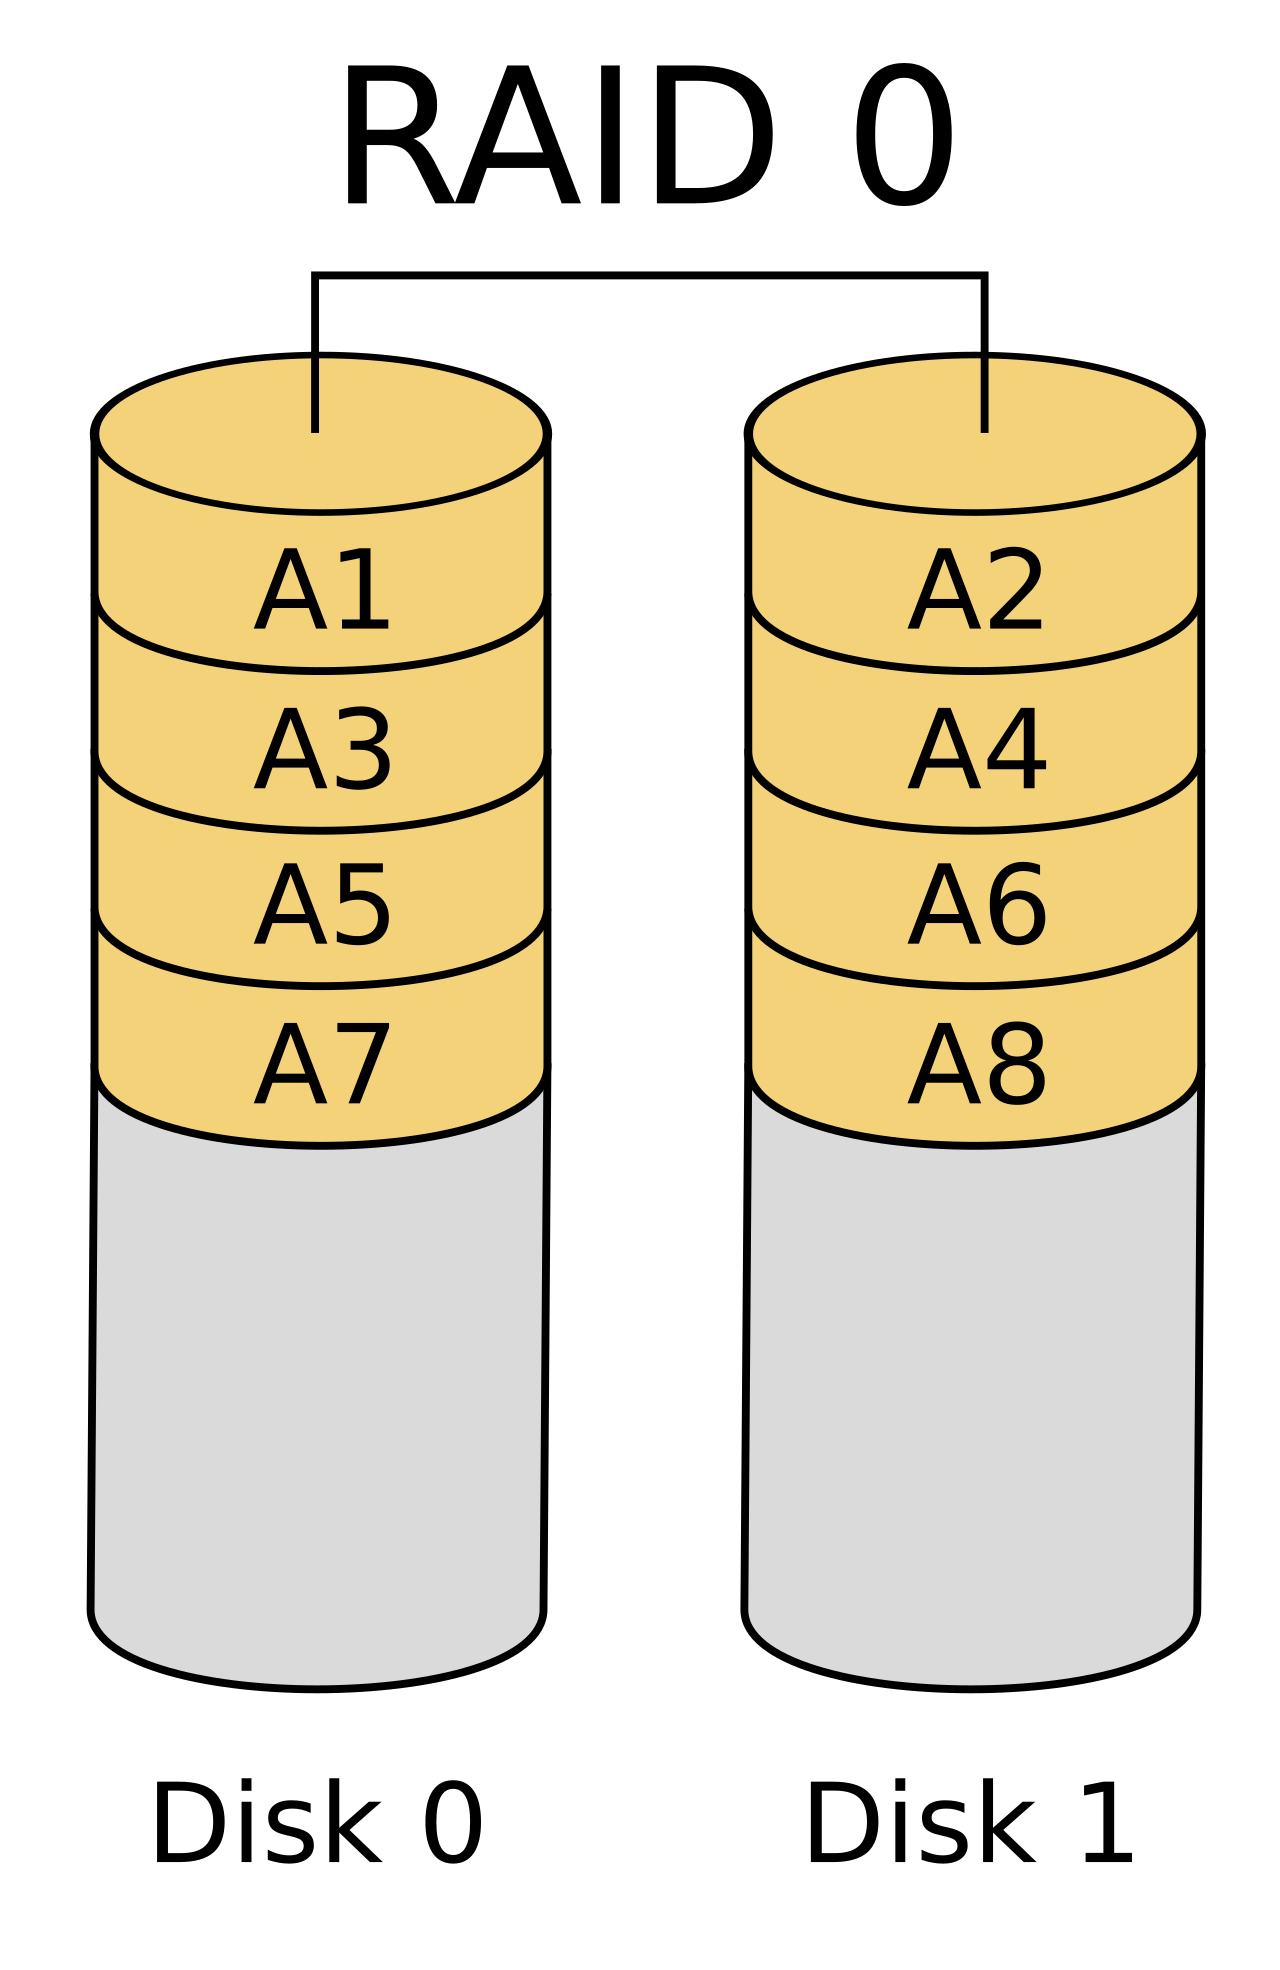
\includegraphics[width=1\linewidth]{assets/RAID_0.png}
    \end{minipage}
\end{figure}

\subsubsection*{RAID 1}
\begin{figure}[H]
    \centering
    \begin{minipage}{0.8\textwidth}
        Prevede la duplicazione di tutti i dati in più dischi, in questo modo si introduce una \textit{ridondanza} che aumenta notevolmente l'affidabilità del sistema.
        La lettura avviene in parallelo, ma la scrittura avviene alla velocità del disco più lento.

    \end{minipage}
    \hfill
    \begin{minipage}{0.15\textwidth}
        \centering
        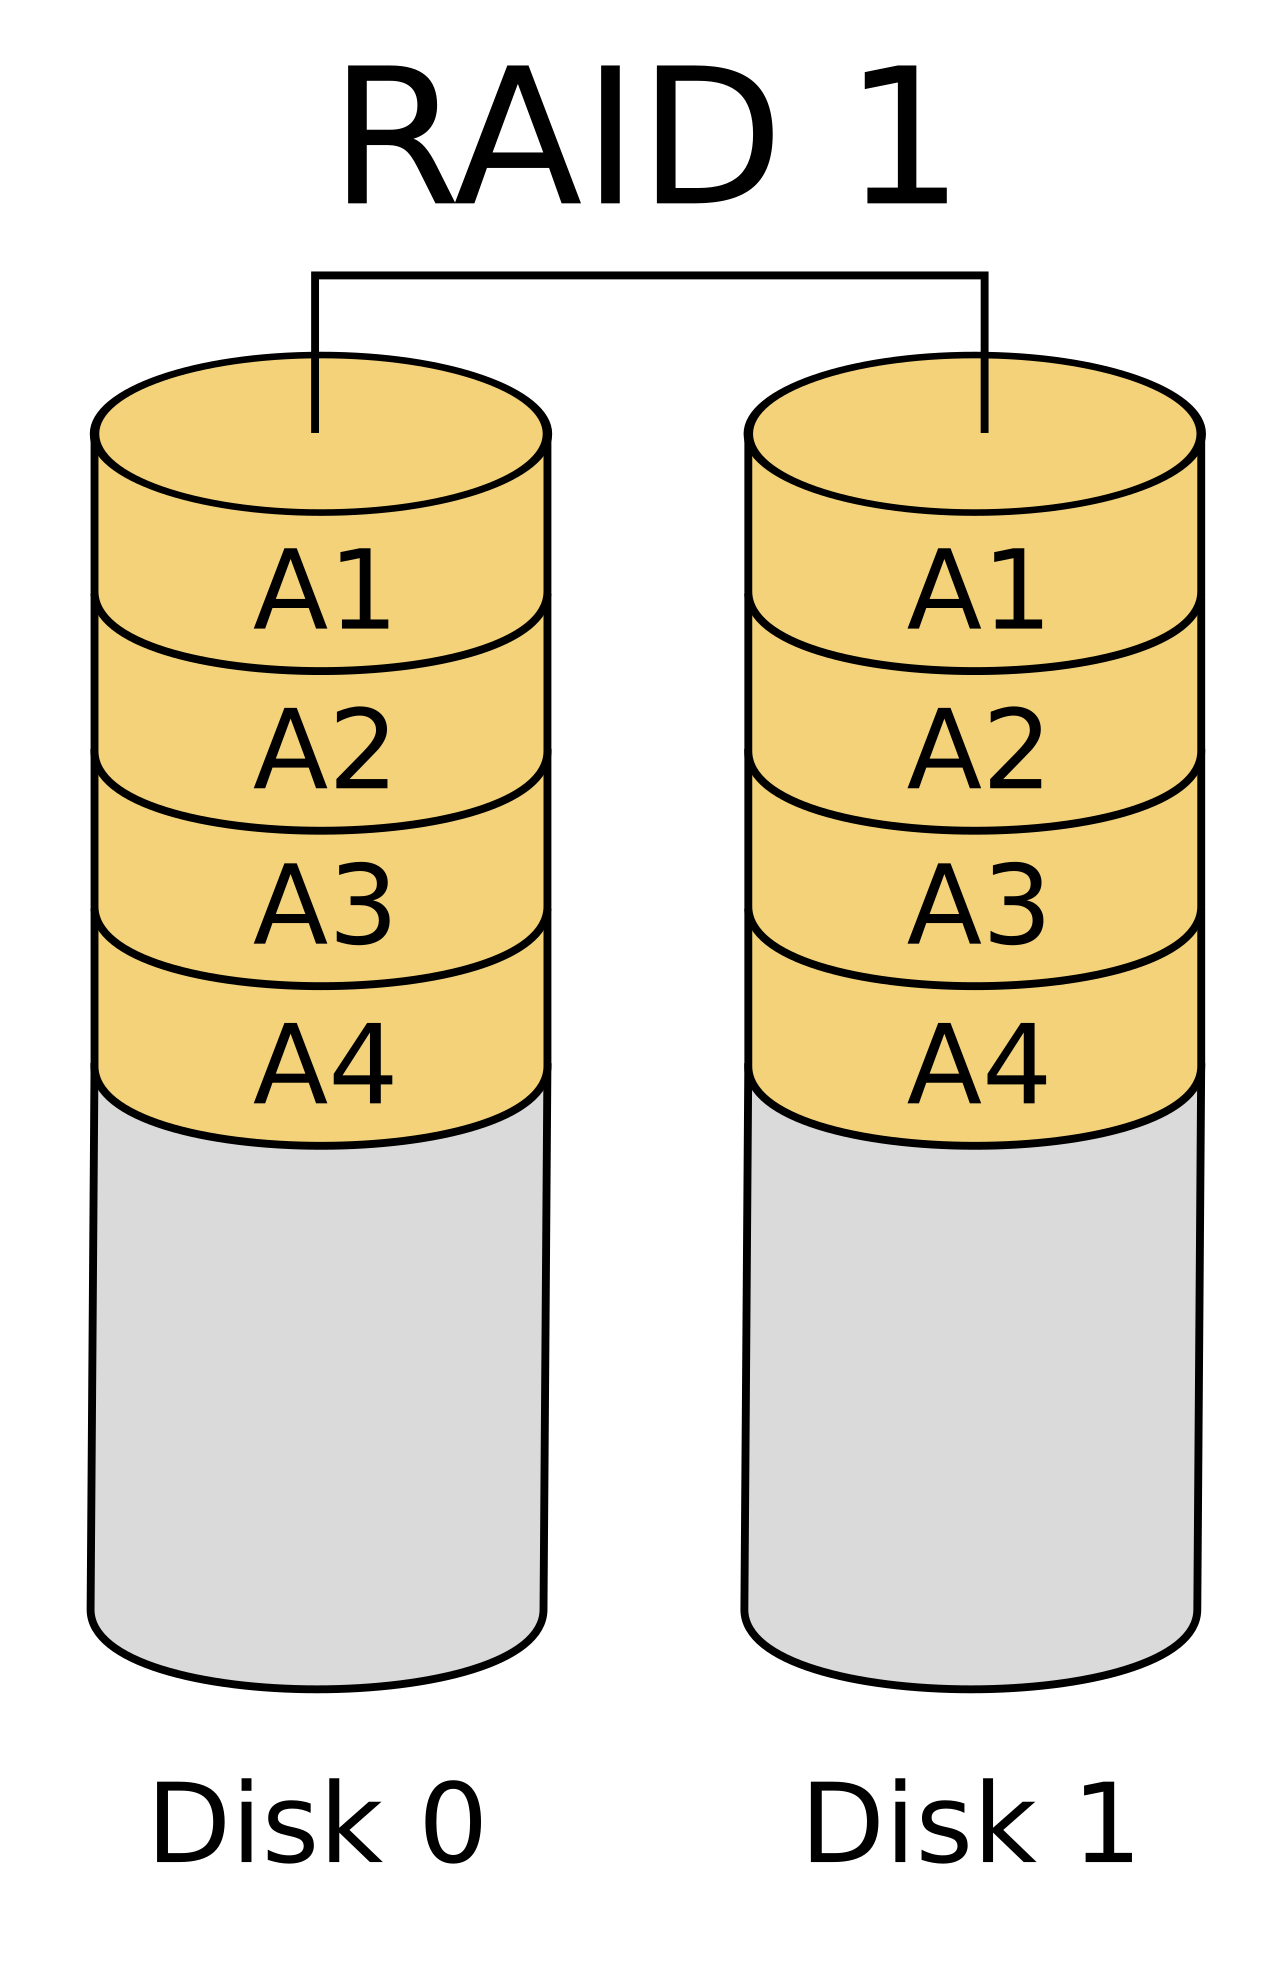
\includegraphics[width=1\linewidth]{assets/RAID_1.png}
    \end{minipage}
\end{figure}

\begin{note}
    RAID 0 e 1 vengono spesso utilizzati in combinazione per ottenere una combinazione dei loro vantaggi.

    \begin{figure}[H]
        \centering
        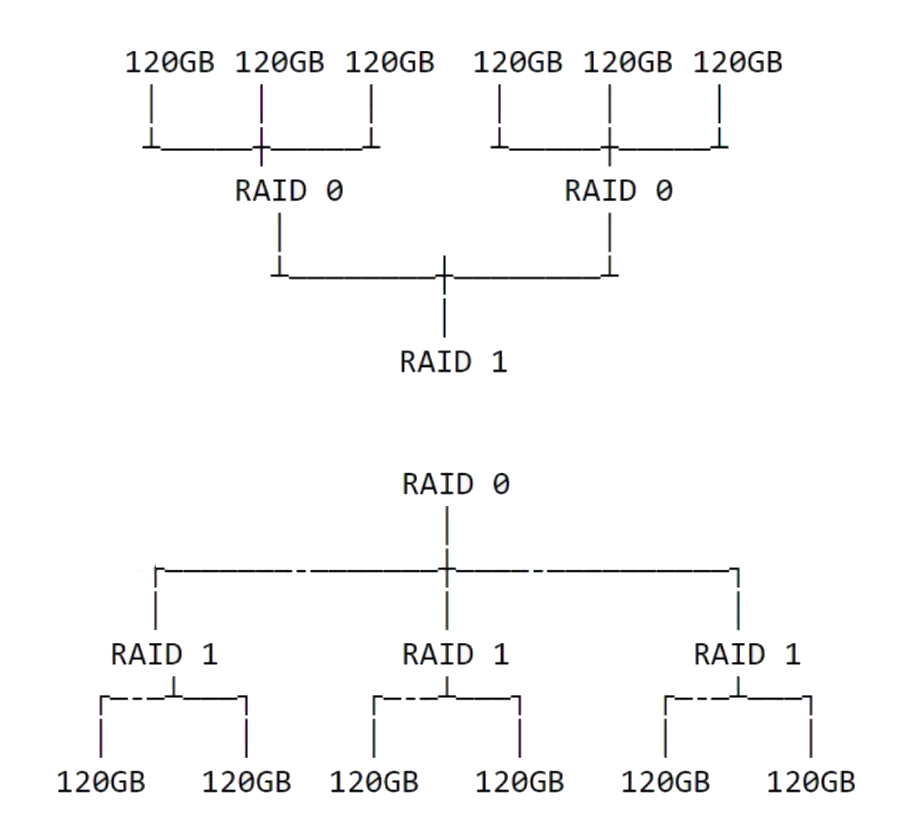
\includegraphics[width=0.4\linewidth]{assets/RAID01.png}
    \end{figure}
\end{note}

\subsubsection*{RAID 2}
\begin{figure}[H]
    \centering
    \begin{minipage}{0.65\textwidth}
        Architettura poco diffusa a livello commerciale, striping a livello di bit, movimento parallelo delle testine. Gli errori vengono rilevati mediante codici di Hamming. Questo permette di rilevare sia l'errore che il disco problematico.

        Il numero di dischi di parità è uguale al $\log_2$ del numero totale di dischi, arrotondato per eccesso.
    \end{minipage}
    \hfill
    \begin{minipage}{0.3\textwidth}
        \centering
        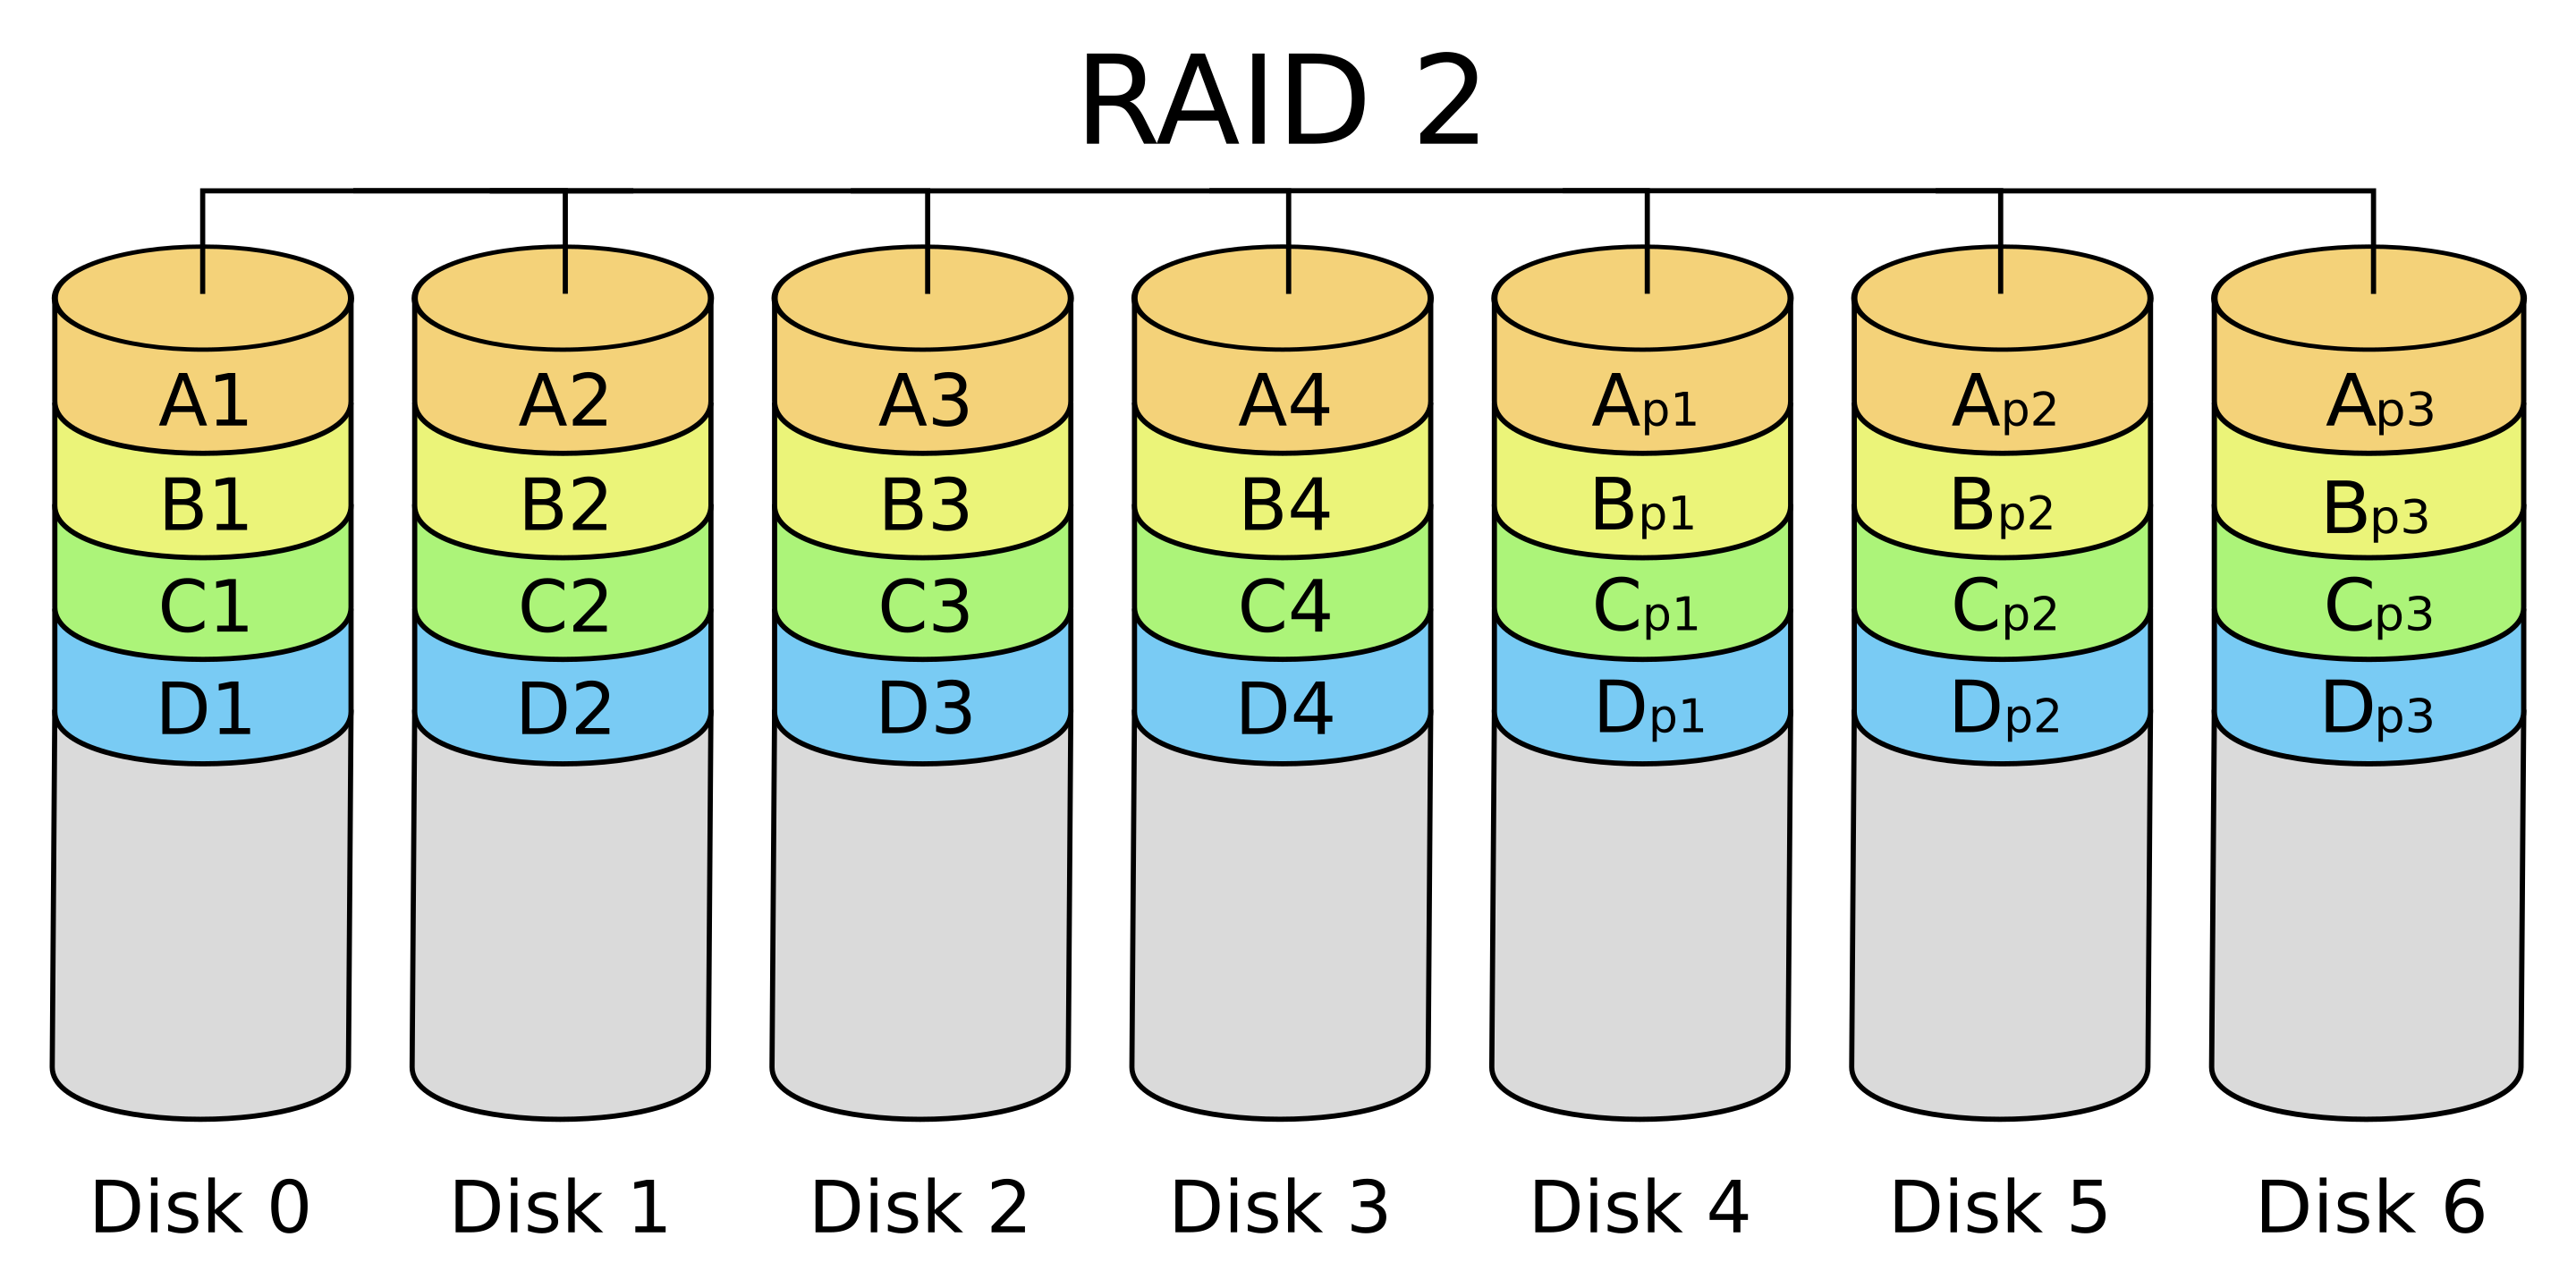
\includegraphics[width=1\linewidth]{assets/RAID_2.png}
    \end{minipage}
\end{figure}

\subsubsection*{RAID 3}
\begin{figure}[H]
    \centering
    \begin{minipage}{0.65\textwidth}
        Funzionamento simile a RAID 2, striping a livello di bit e movimento parallelo delle testine.

        Un disco viene utilizzato per la parità, permettendo al sistema di accettare una perdita di un disco.
    \end{minipage}
    \hfill
    \begin{minipage}{0.3\textwidth}
        \centering
        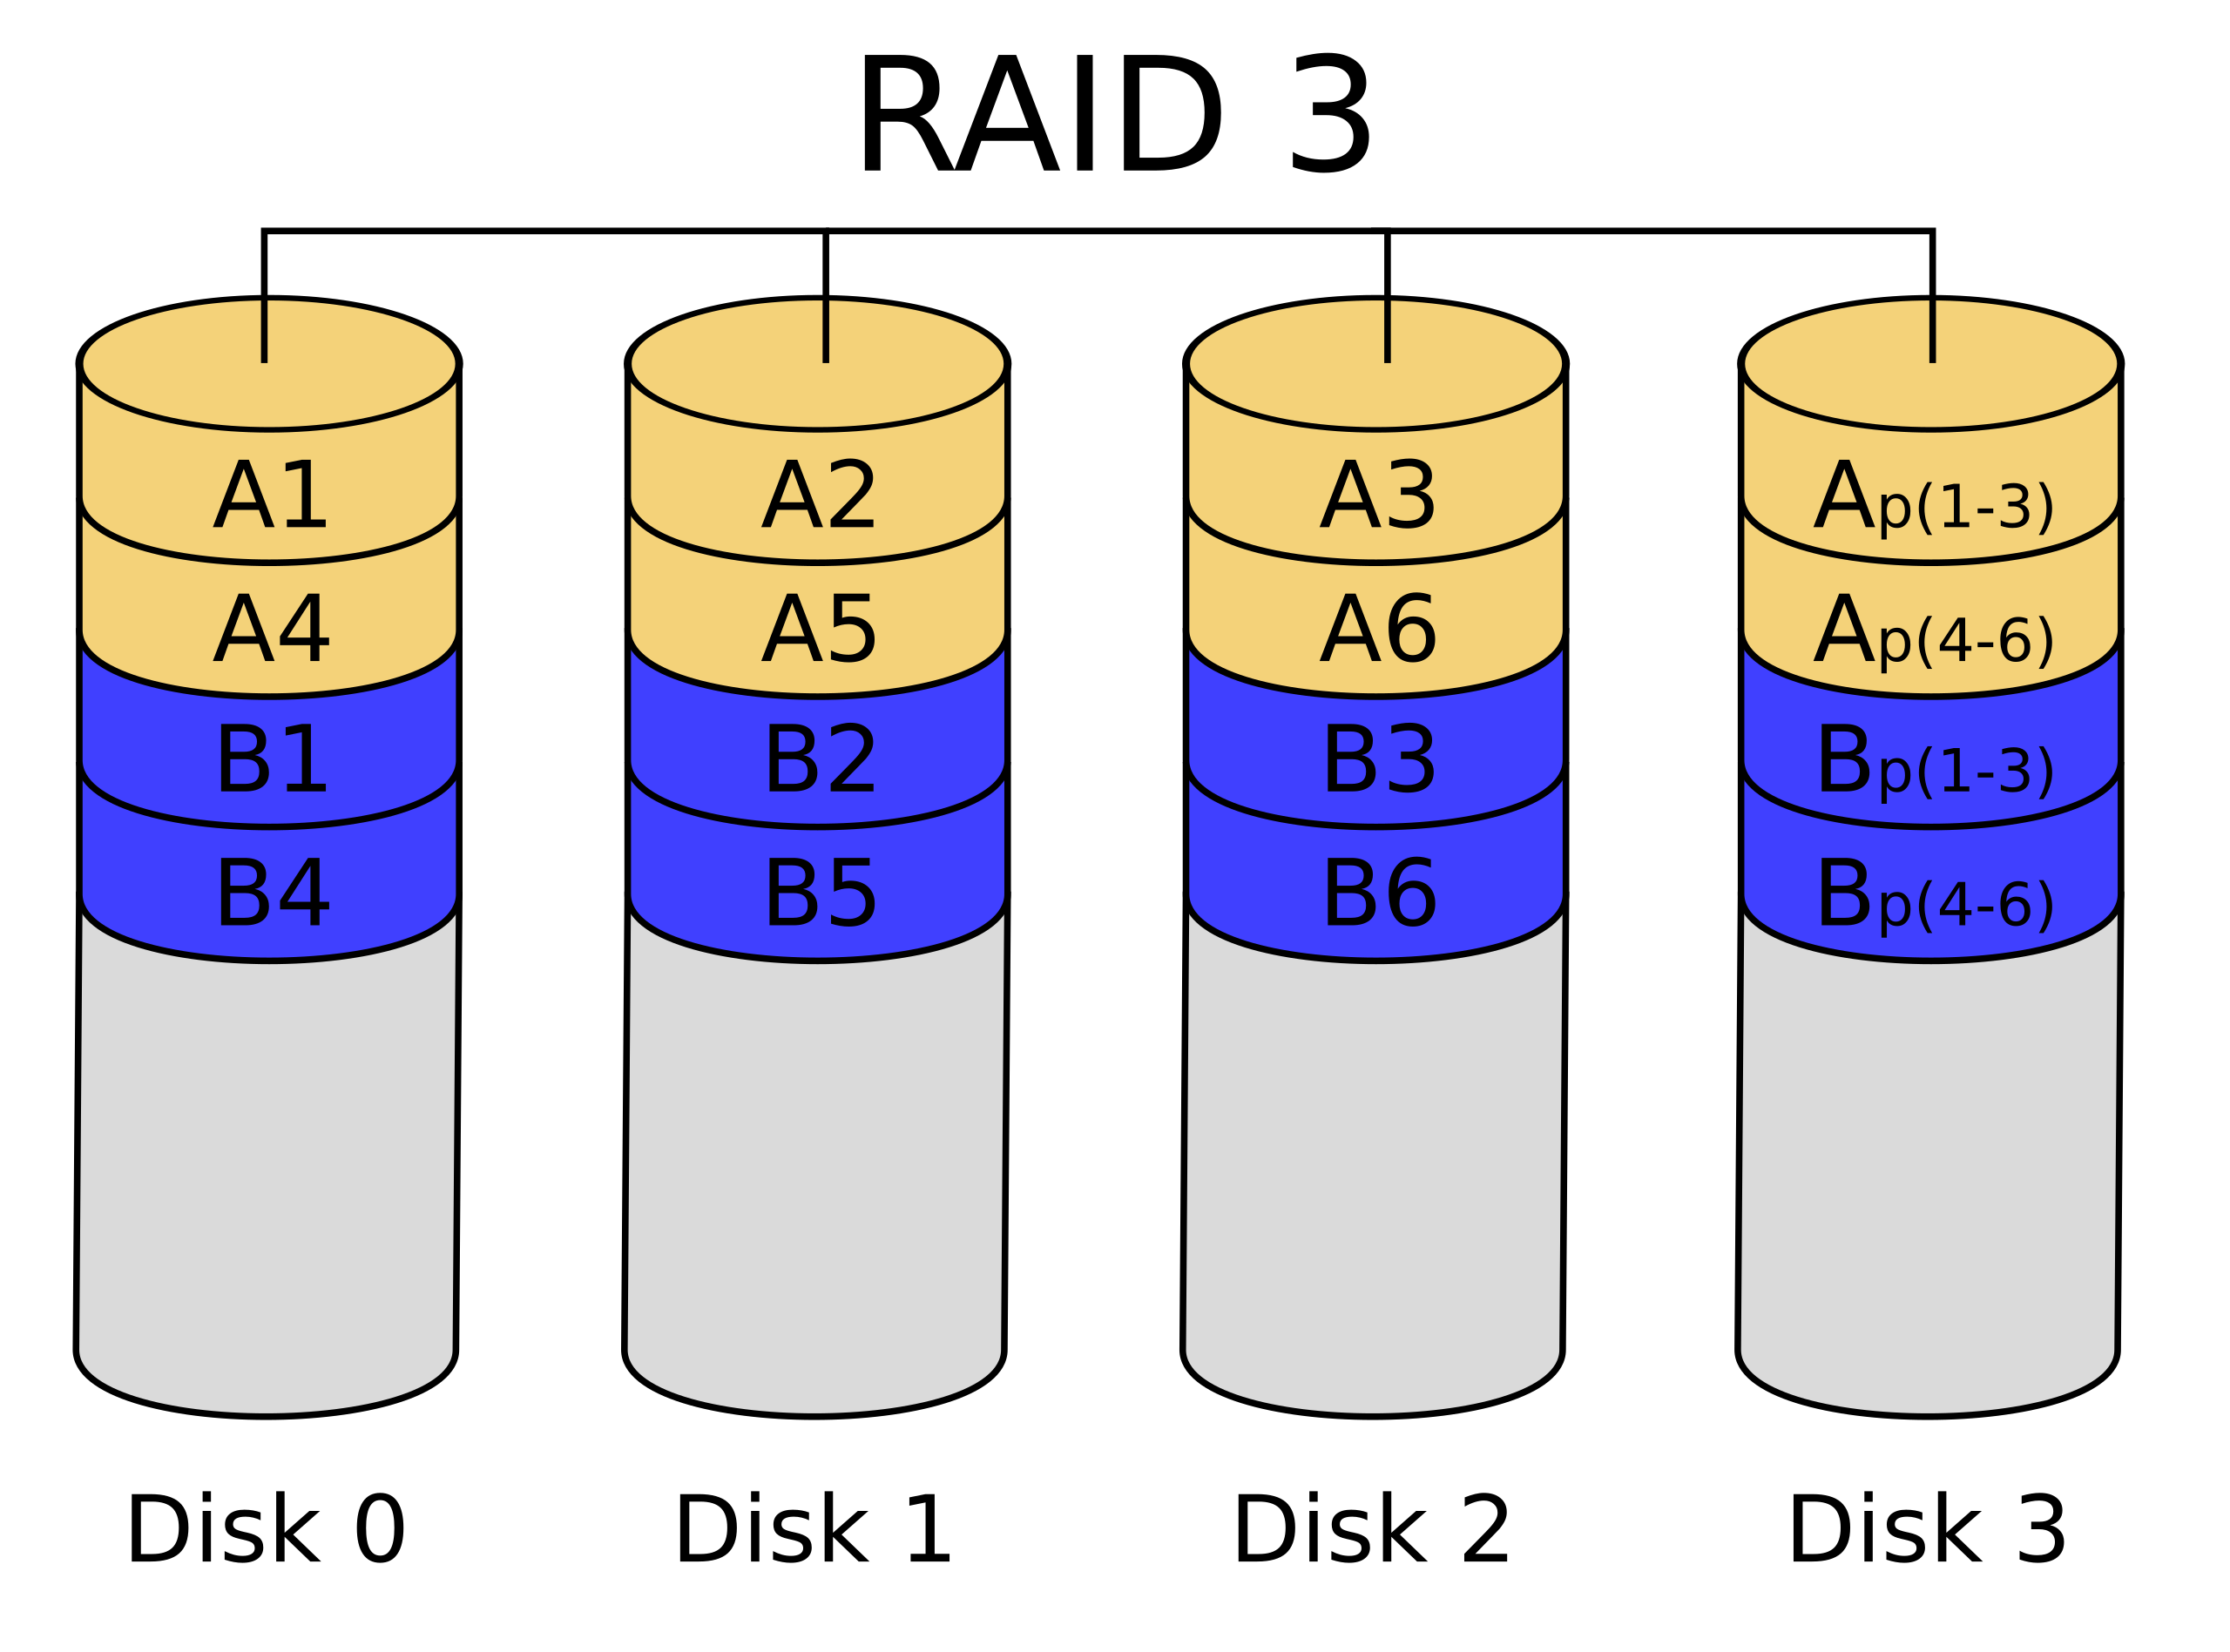
\includegraphics[width=1\linewidth]{assets/RAID_3.png}
    \end{minipage}
\end{figure}

\subsubsection*{RAID 4}
\begin{figure}[H]
    \centering
    \begin{minipage}{0.65\textwidth}
        Striping a livello di blocco, testine indipendenti e utilizzo di un solo disco di parità.
        In questo modo le letture piccole richiedono un solo disco, e possono essere svolte in modo parallelo. Mentre le scritture richiedono anche l'accesso al disco di parità.
    \end{minipage}
    \hfill
    \begin{minipage}{0.3\textwidth}
        \centering
        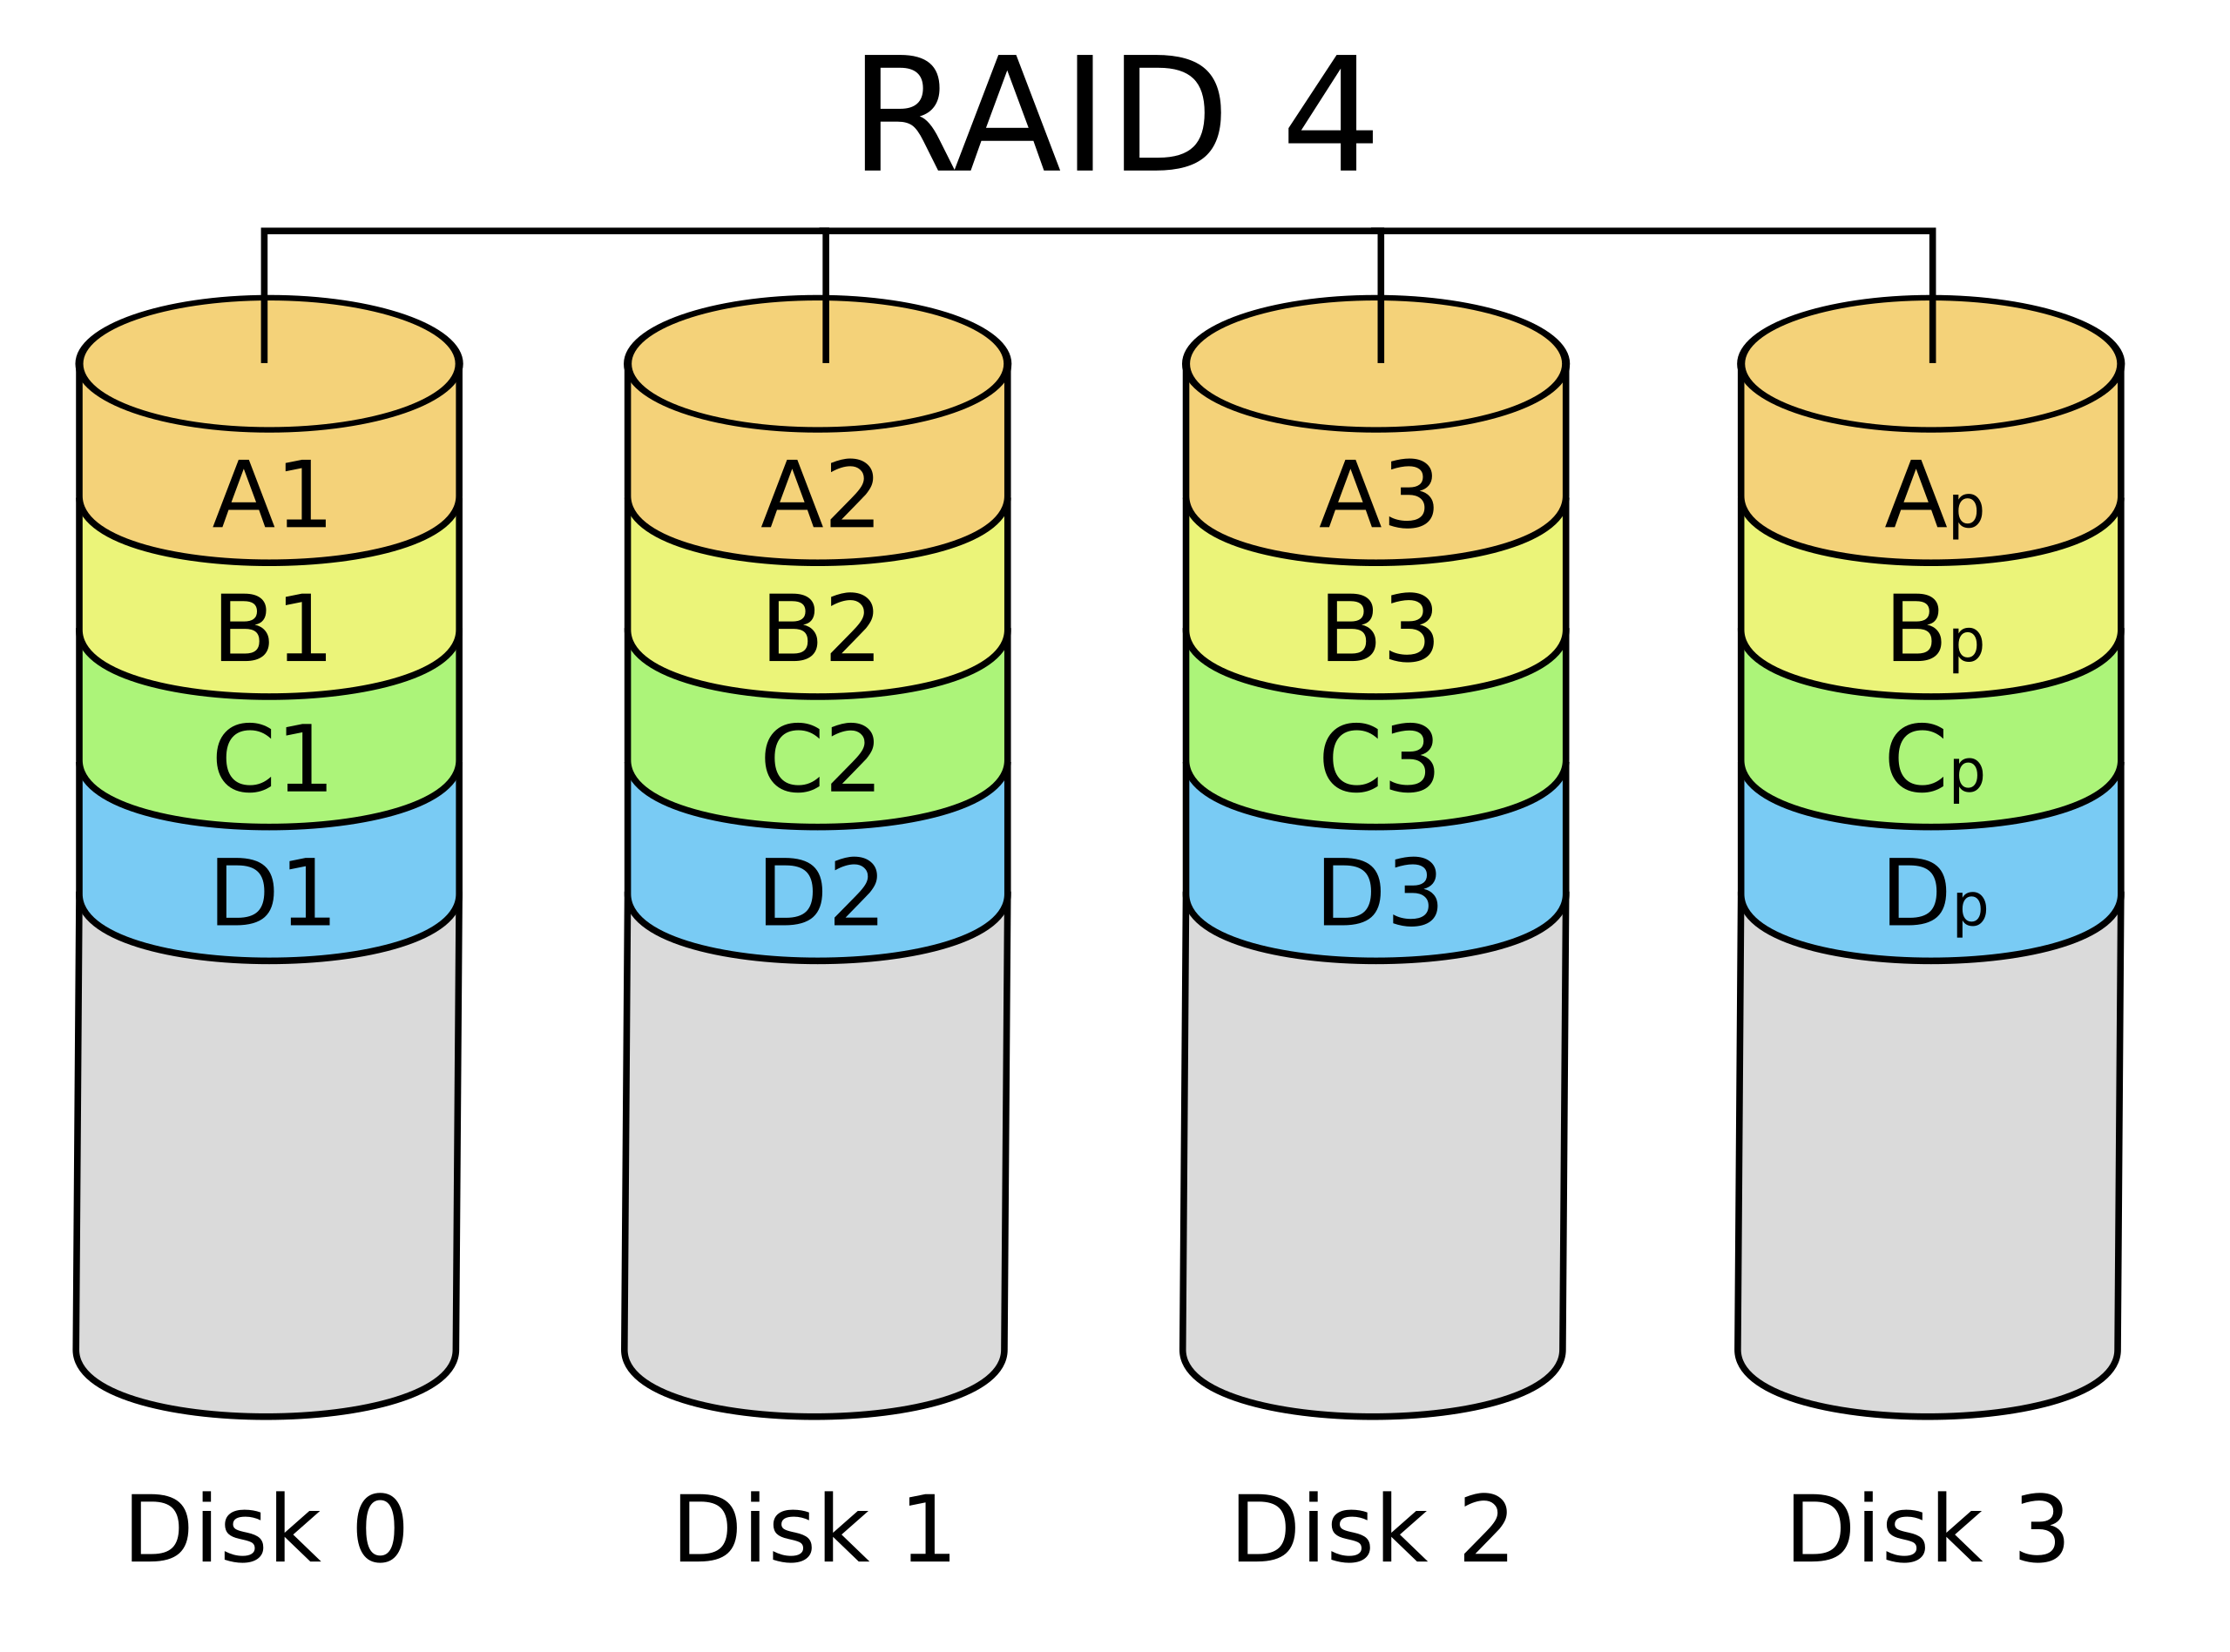
\includegraphics[width=1\linewidth]{assets/RAID_4.png}
    \end{minipage}
\end{figure}

\subsubsection*{RAID 5}
\begin{figure}[H]
    \centering
    \begin{minipage}{0.65\textwidth}
        Sia RAID 3 che RAID 4 hanno un solo disco di parity, il che significa che è un bottleneck in quanto limita le operazioni parallele che possono essere svolte dai dischi. Il RAID 5 distribuisce questi bit su più dischi, migliorando le prestazioni. Inoltre ha striping a livello di blocco con testine indipendenti.
    \end{minipage}
    \hfill
    \begin{minipage}{0.3\textwidth}
        \centering
        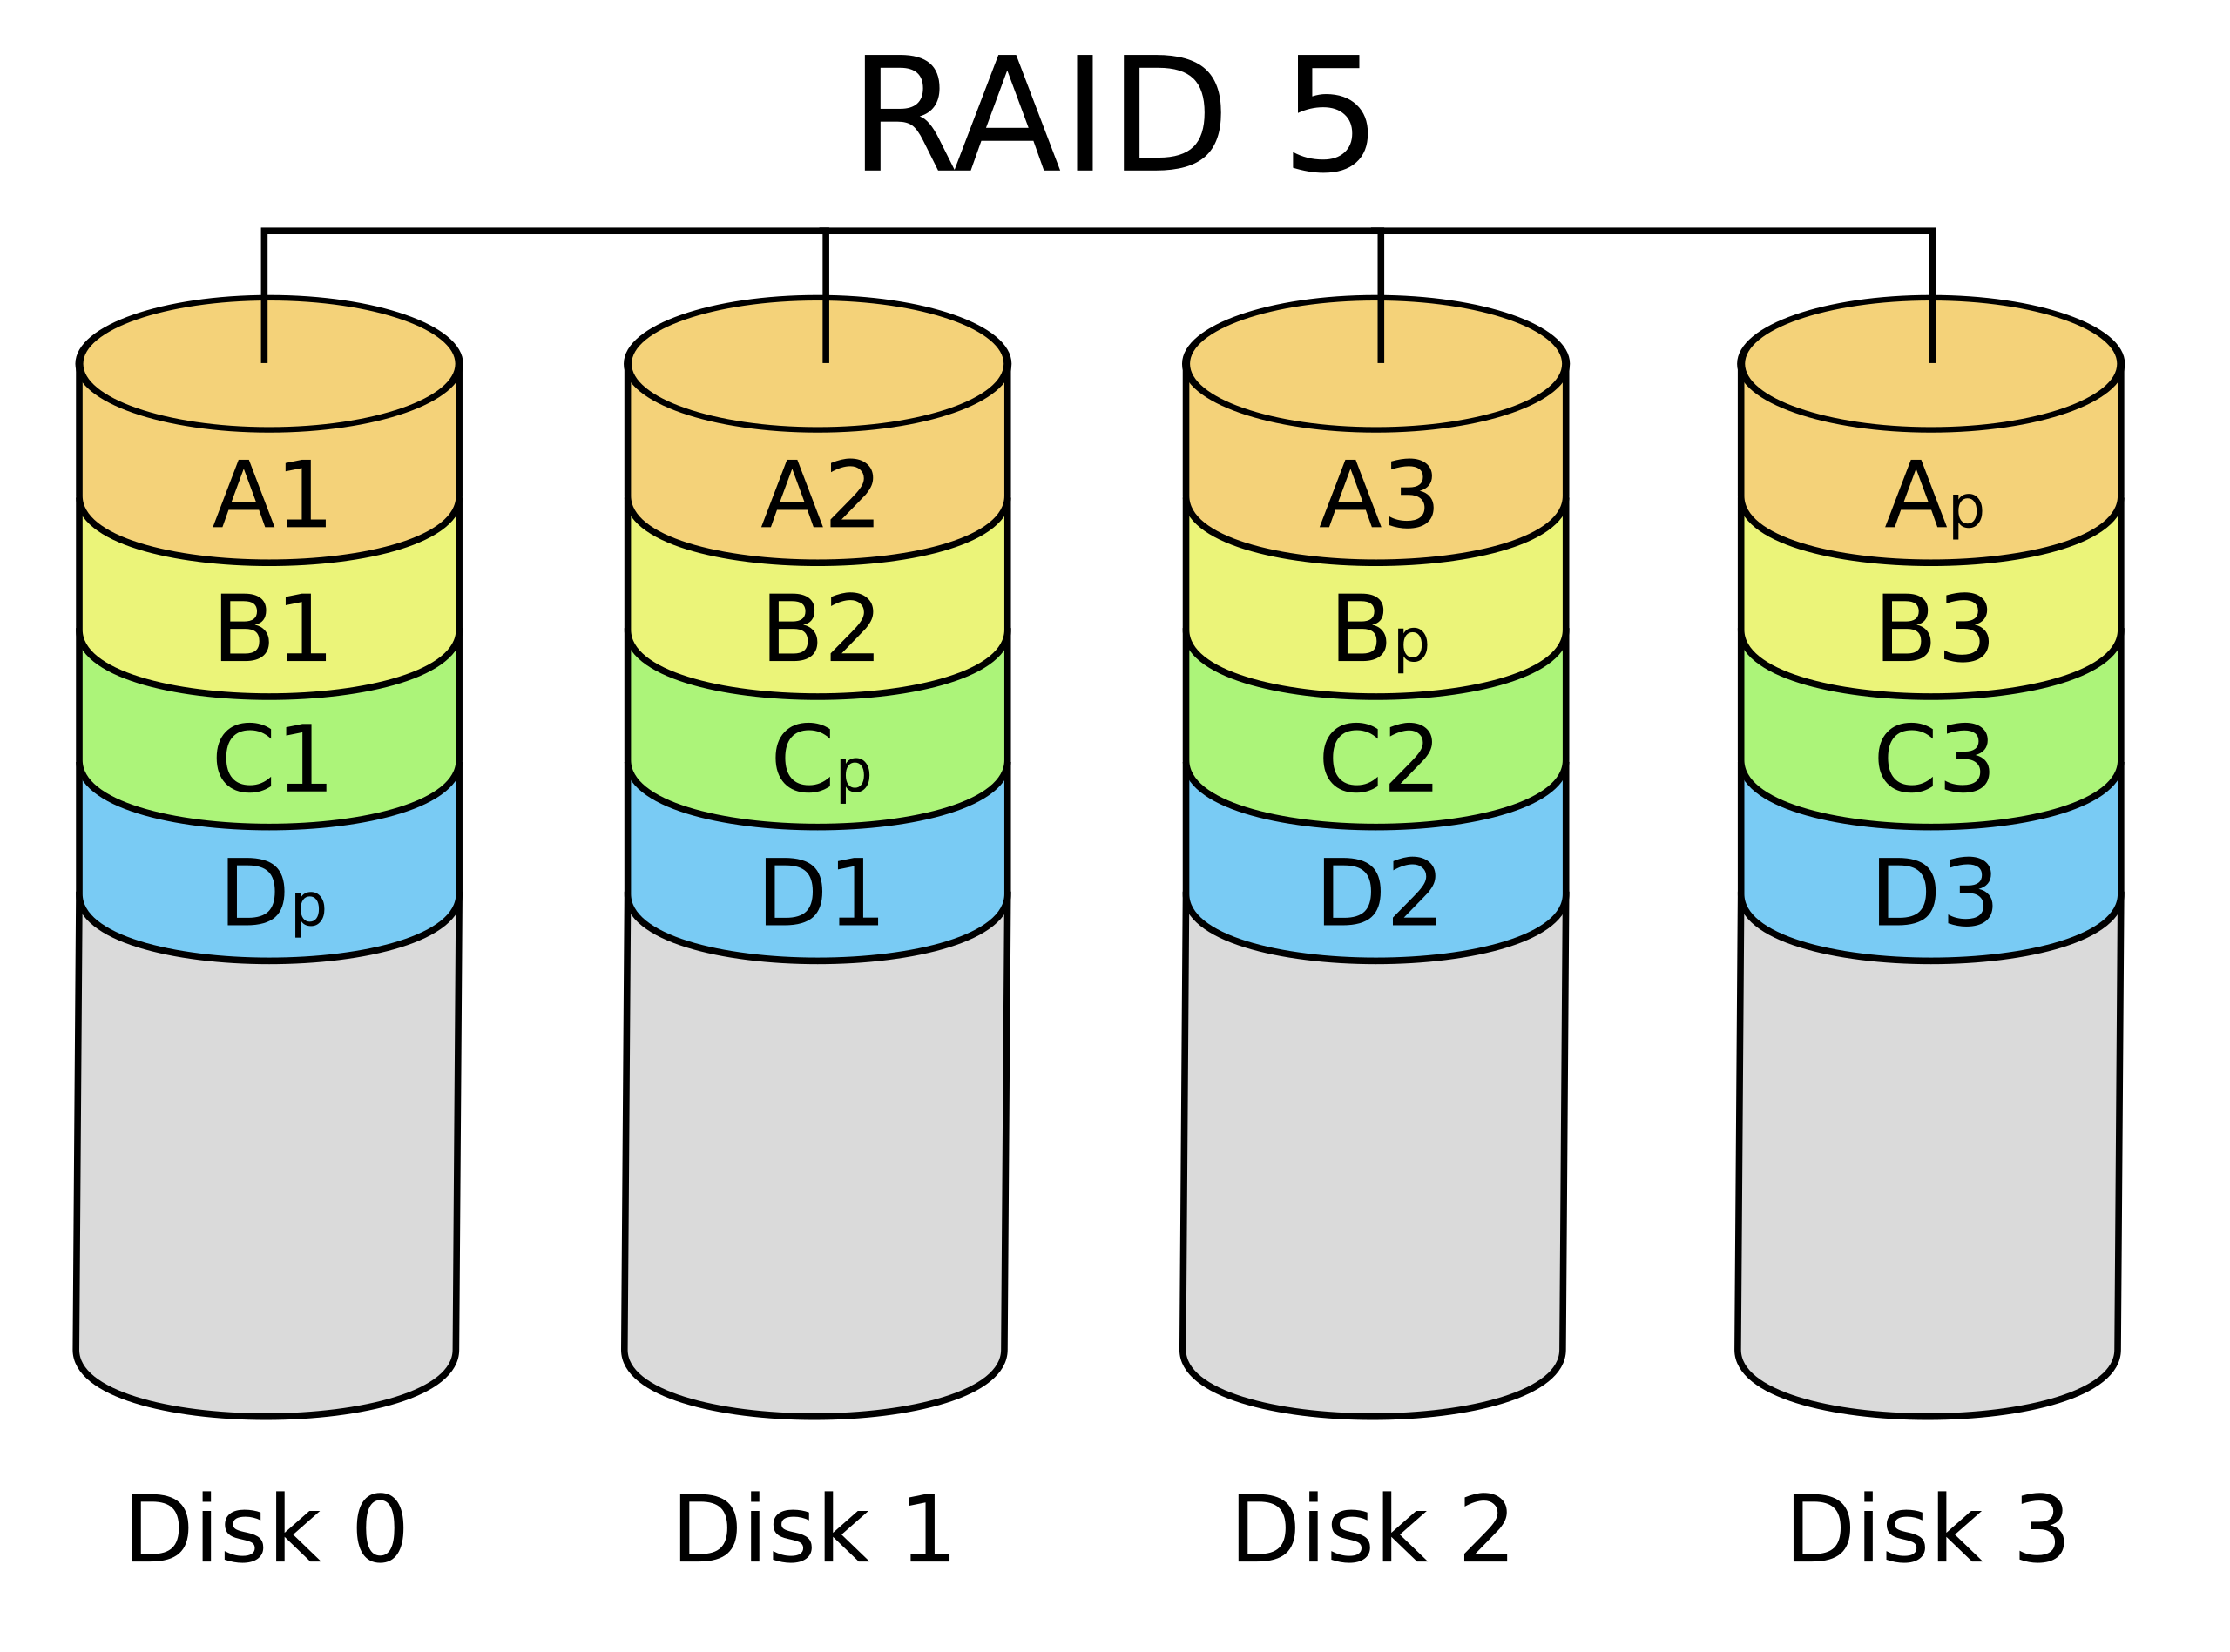
\includegraphics[width=1\linewidth]{assets/RAID_5.png}
    \end{minipage}
\end{figure}

\subsubsection*{RAID 6}
\begin{figure}[H]
    \centering
    \begin{minipage}{0.65\textwidth}
        La limitazione del RAID 5 è che è in grado di tollerare la perdita di un solo disco, il RAID 6 aumenta questo margine a 2 dischi.
    \end{minipage}
    \hfill
    \begin{minipage}{0.3\textwidth}
        \centering
        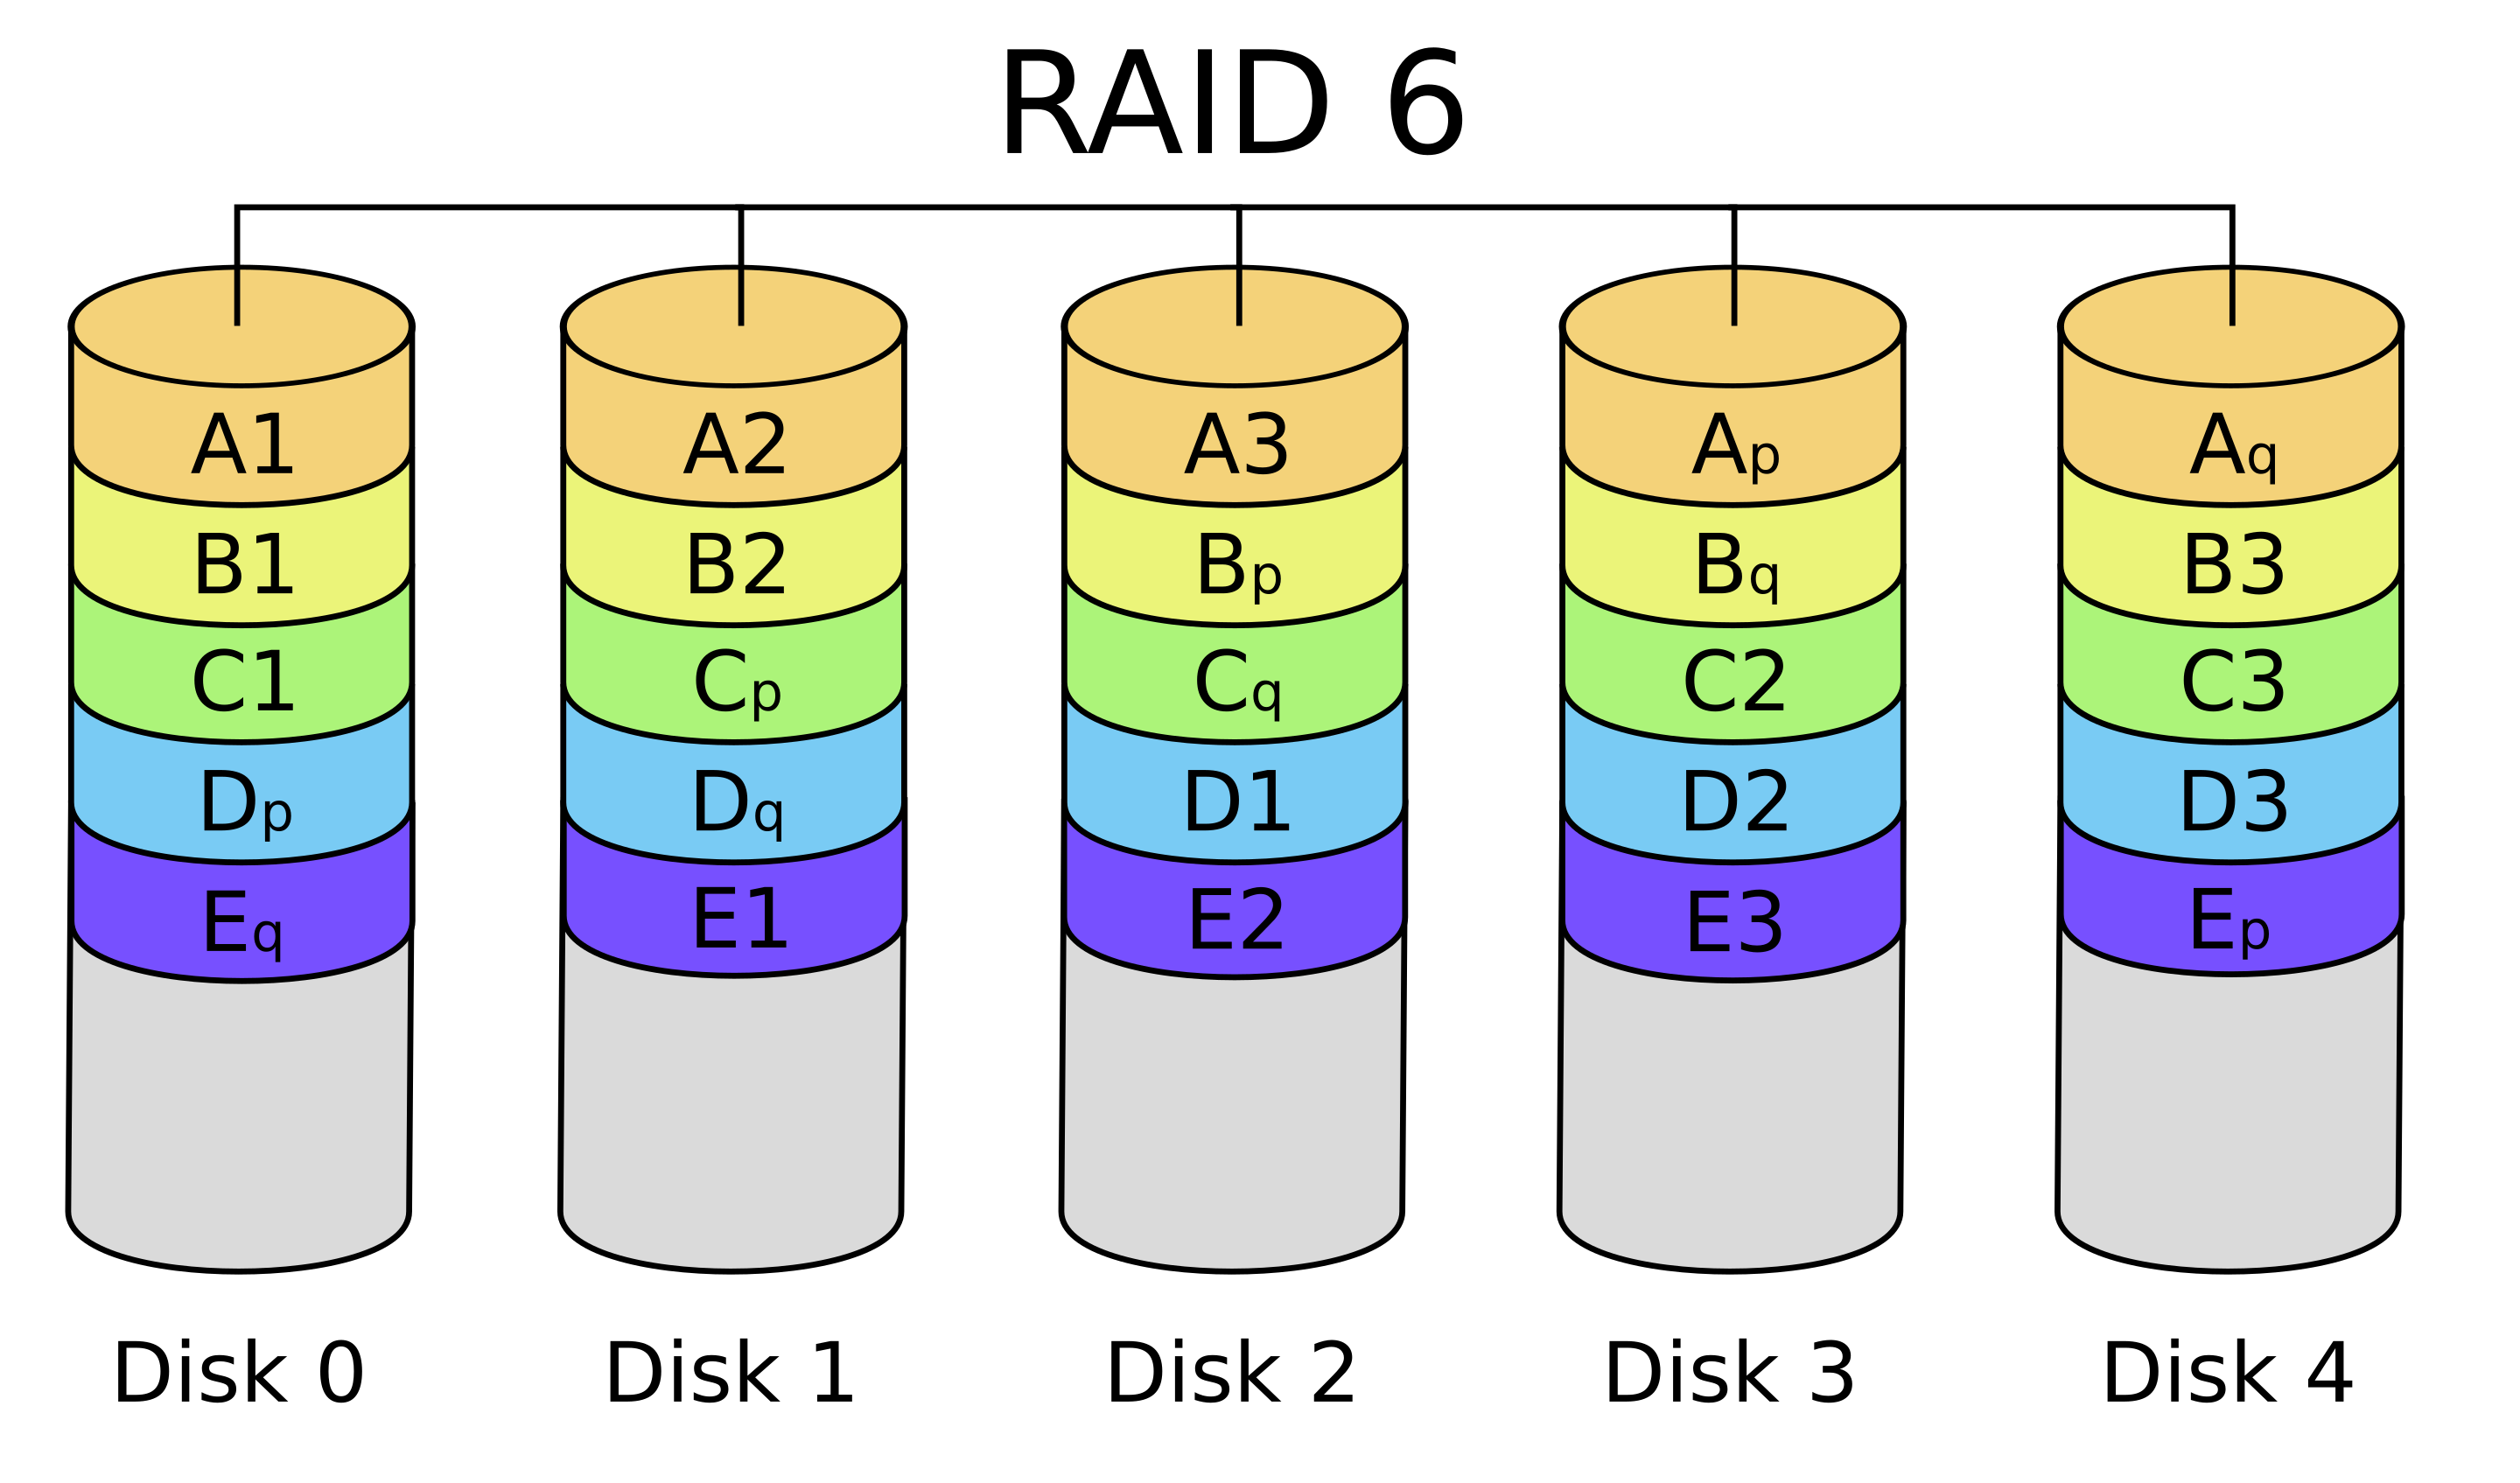
\includegraphics[width=1\linewidth]{assets/RAID_6.png}
    \end{minipage}
\end{figure}
